\section{Results with fixed final state fractions}
\label{app:fixfrac}

\begin{figure}[!h!tb]
  \begin{center}

    \subfigure[$\pt(\mathrm{H})$]{
      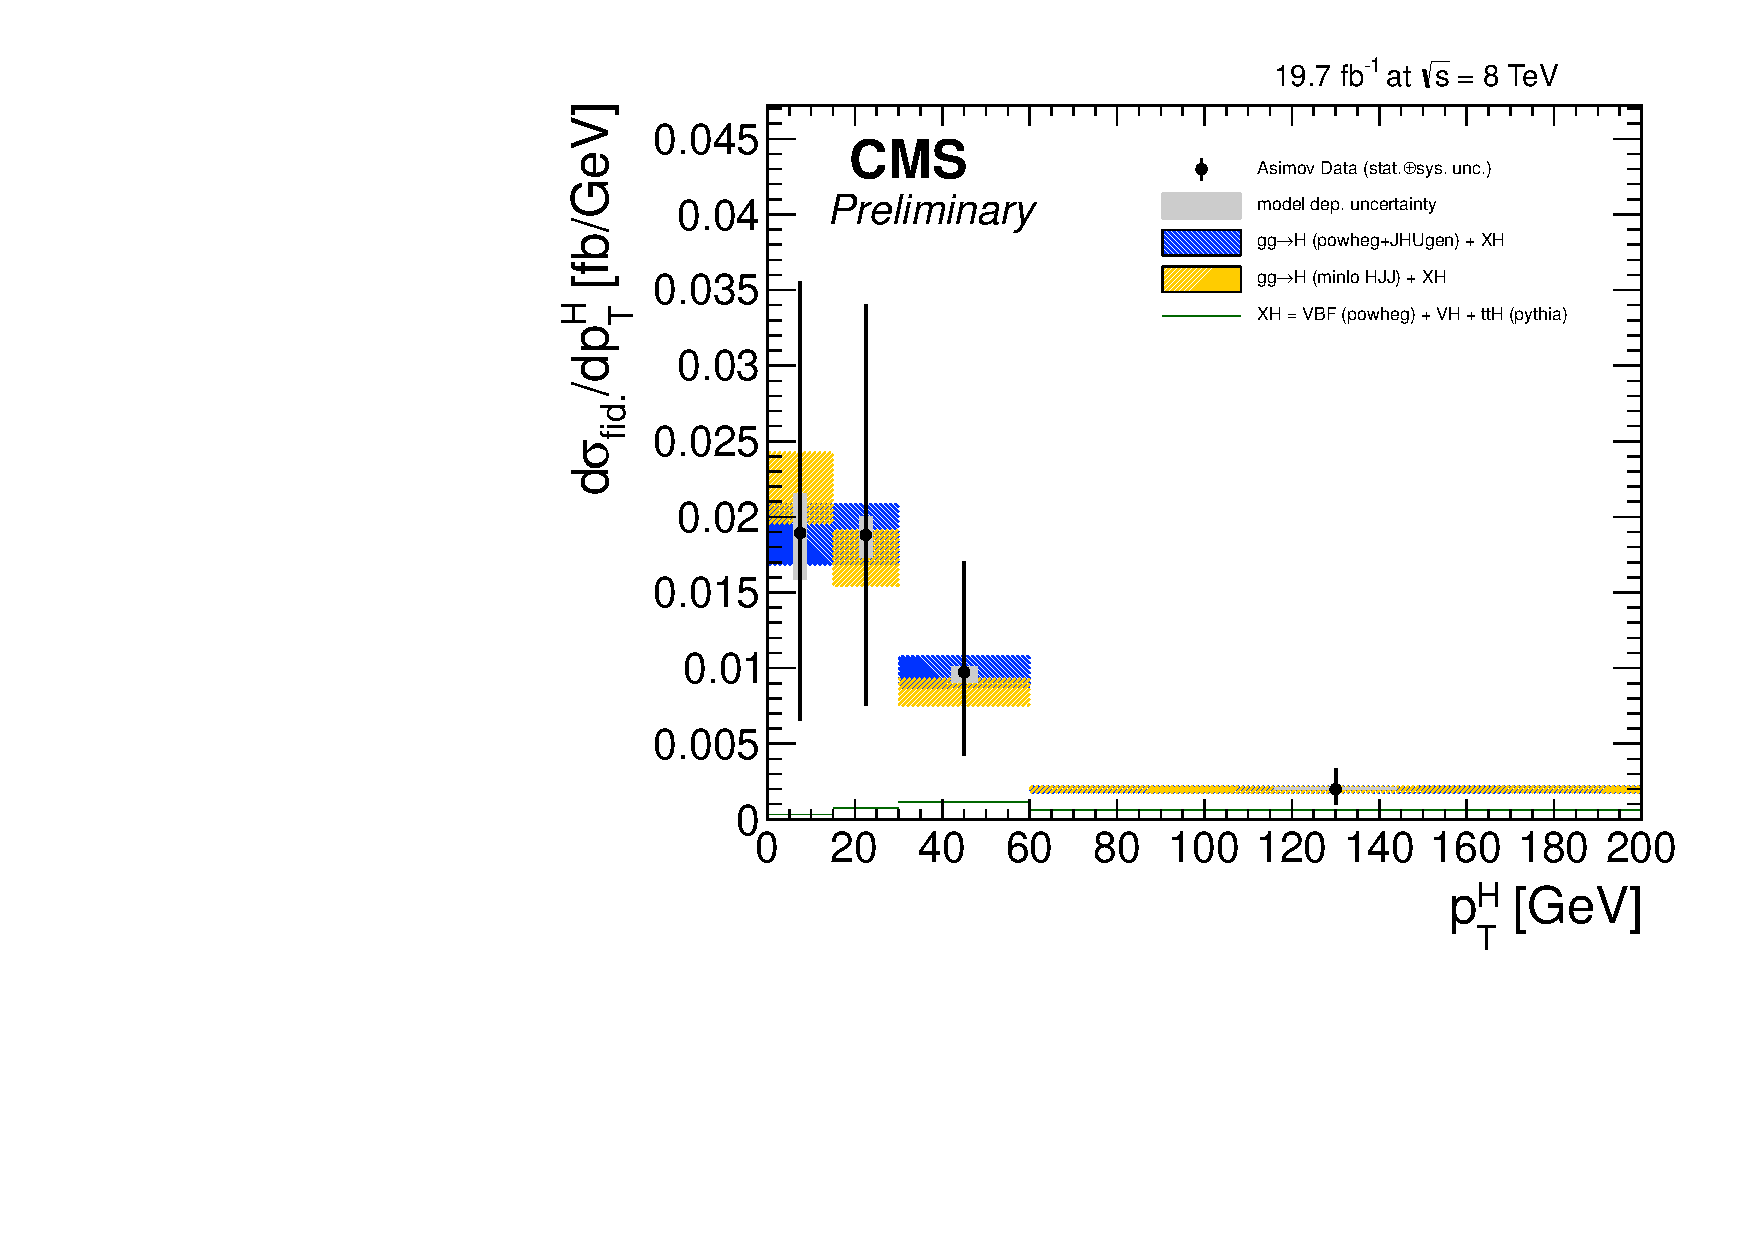
\includegraphics[width=0.48\textwidth,angle=0]{Plots/pT4l_unfoldwith_ggH_powheg15_JHUgen_125_fixfrac.pdf}
      \label{fig:differential-results-fixfrac:a}
    }
    \subfigure[$\mathrm{m}(\mathrm{Z}_{2})$]{
      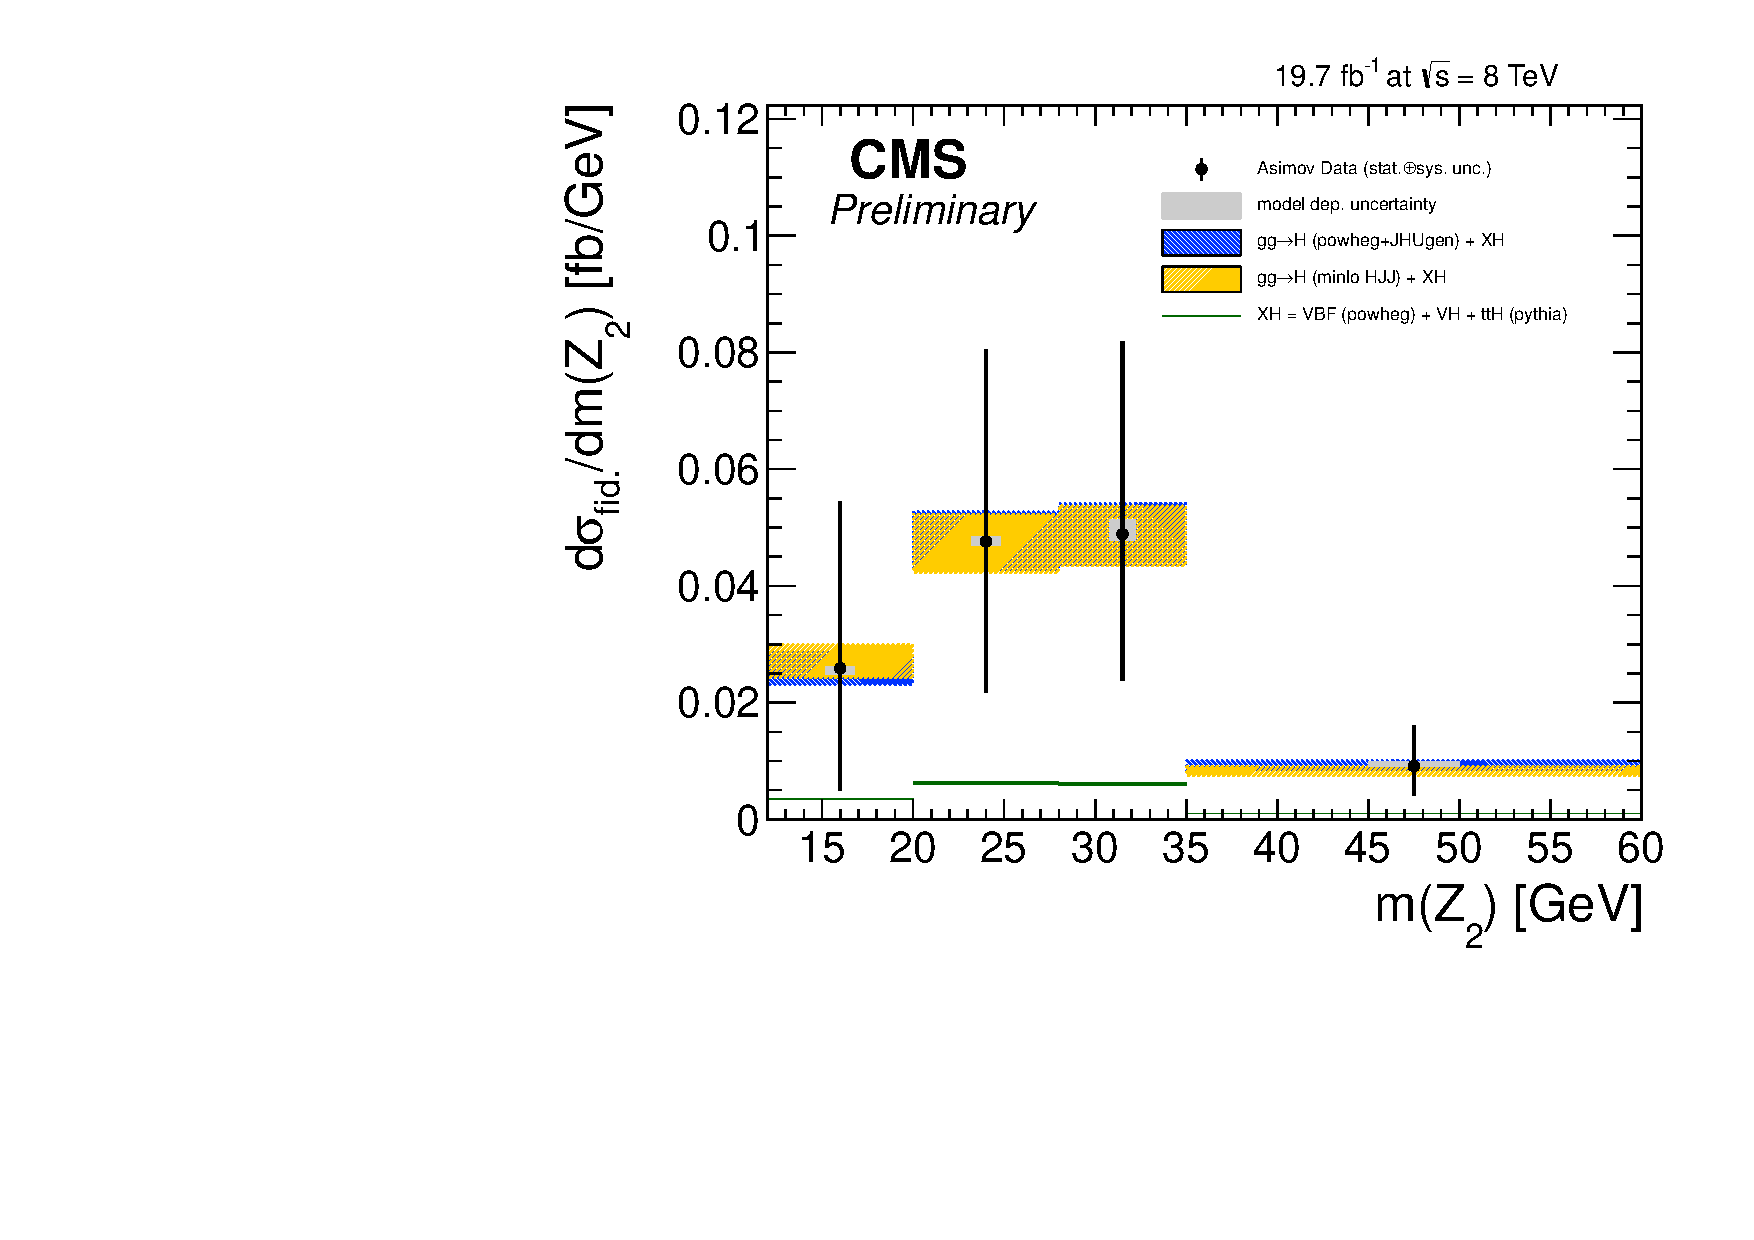
\includegraphics[width=0.48\textwidth,angle=0]{Plots/massZ2_unfoldwith_ggH_powheg15_JHUgen_125_fixfrac.pdf}
      \label{fig:differential-results-fixfrac:b}
    } \\
    \subfigure[$|y(\mathrm{H})|$]{
      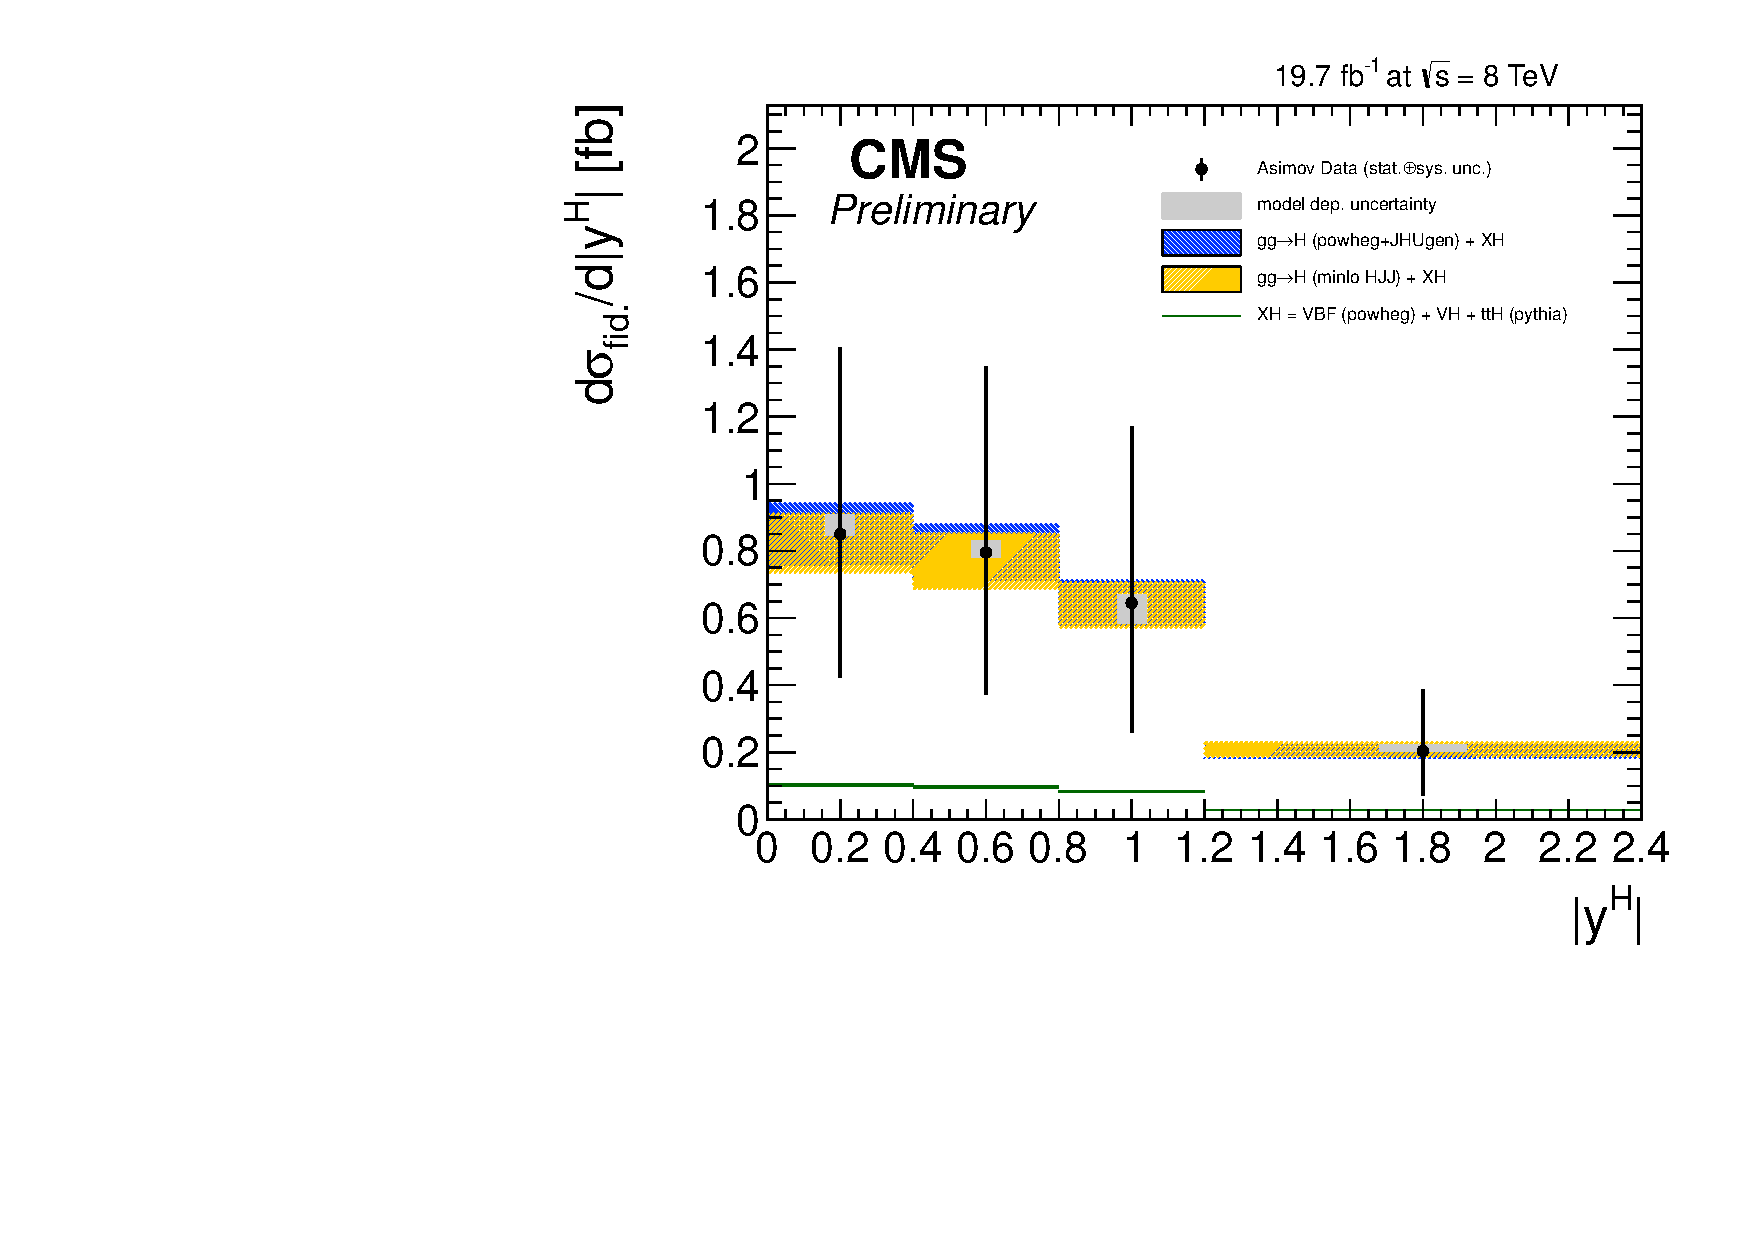
\includegraphics[width=0.48\textwidth,angle=0]{Plots/rapidity4l_unfoldwith_ggH_powheg15_JHUgen_125_fixfrac.pdf}
      \label{fig:differential-results-fixfrac:b}
    }
    \subfigure[$|\cos \theta^{*}|$]{
      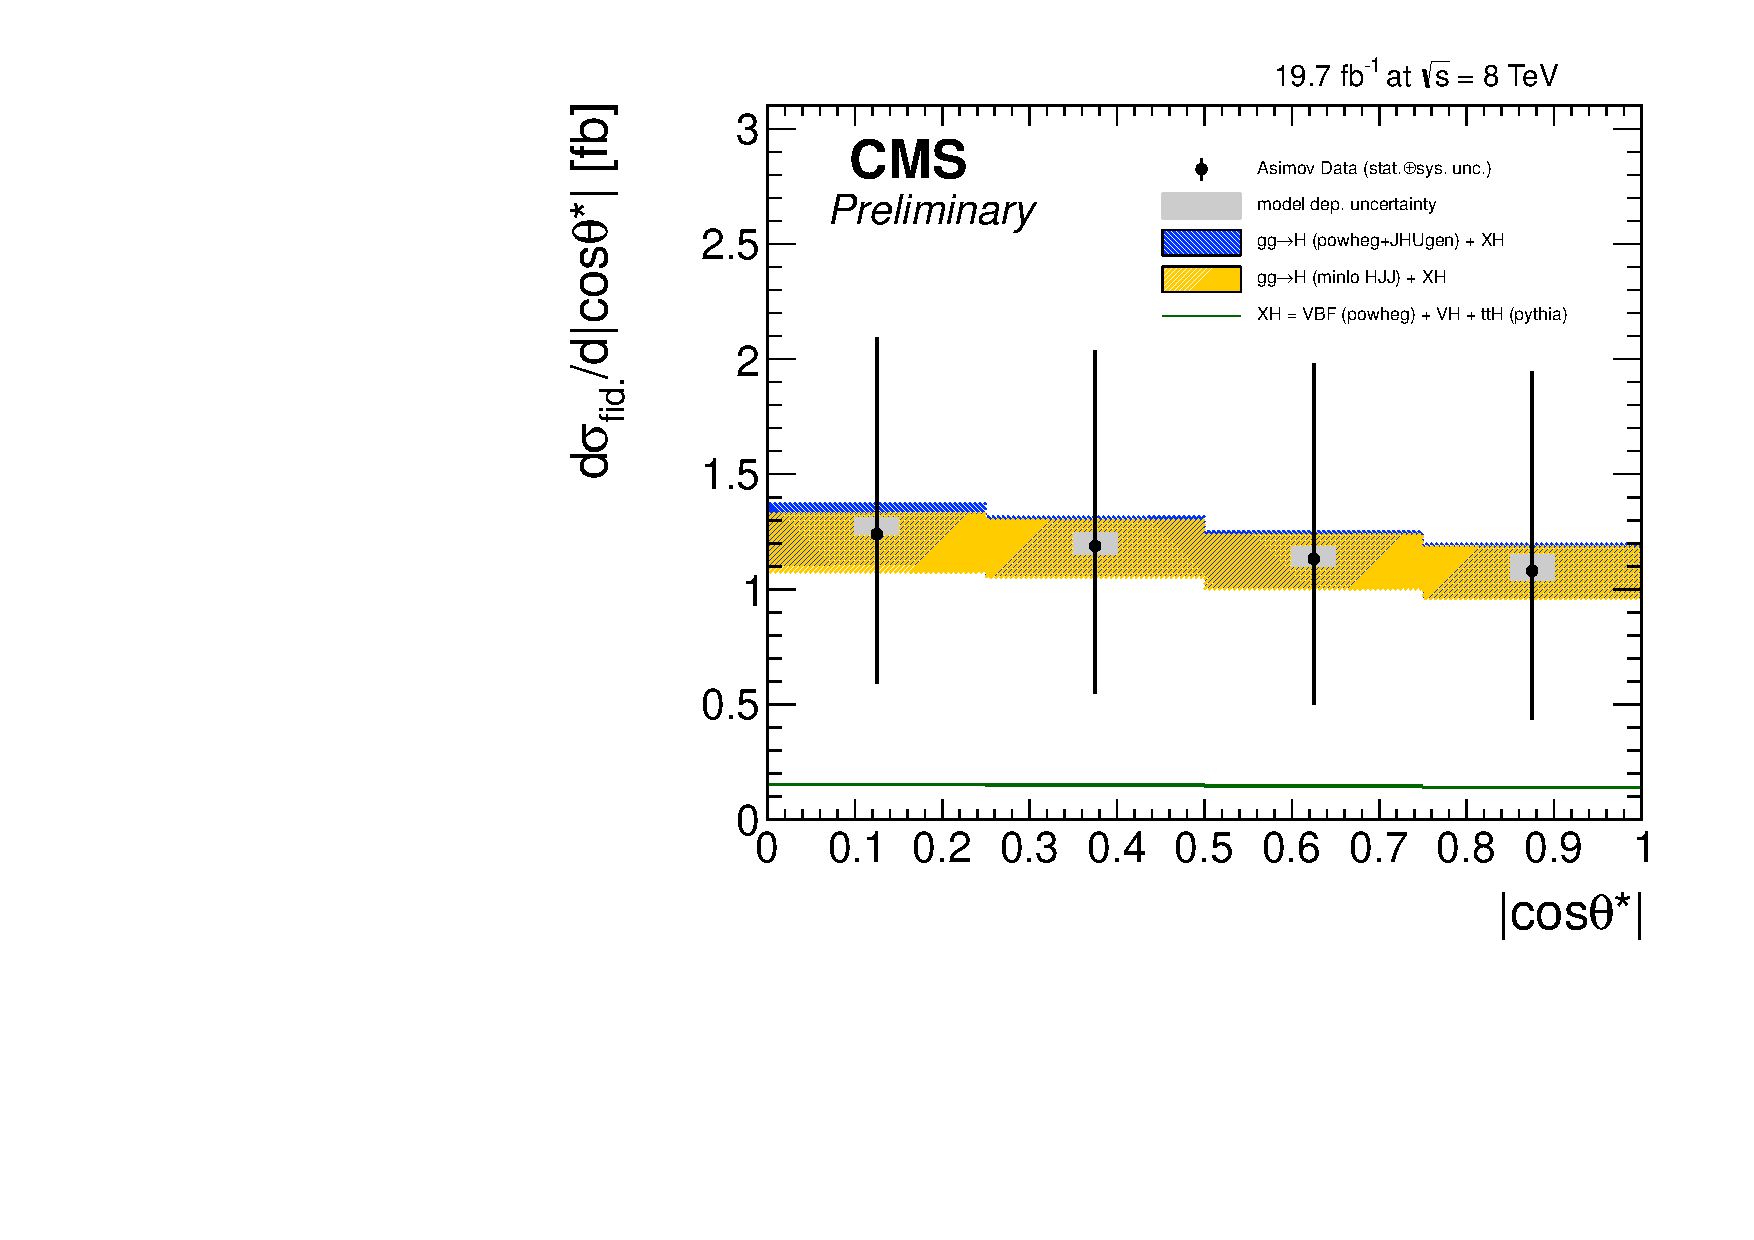
\includegraphics[width=0.48\textwidth,angle=0]{Plots/cosThetaStar_unfoldwith_ggH_powheg15_JHUgen_125_fixfrac.pdf}
      \label{fig:differential-results-fixfrac:c}
    } \\
    \subfigure[N(jets)]{
      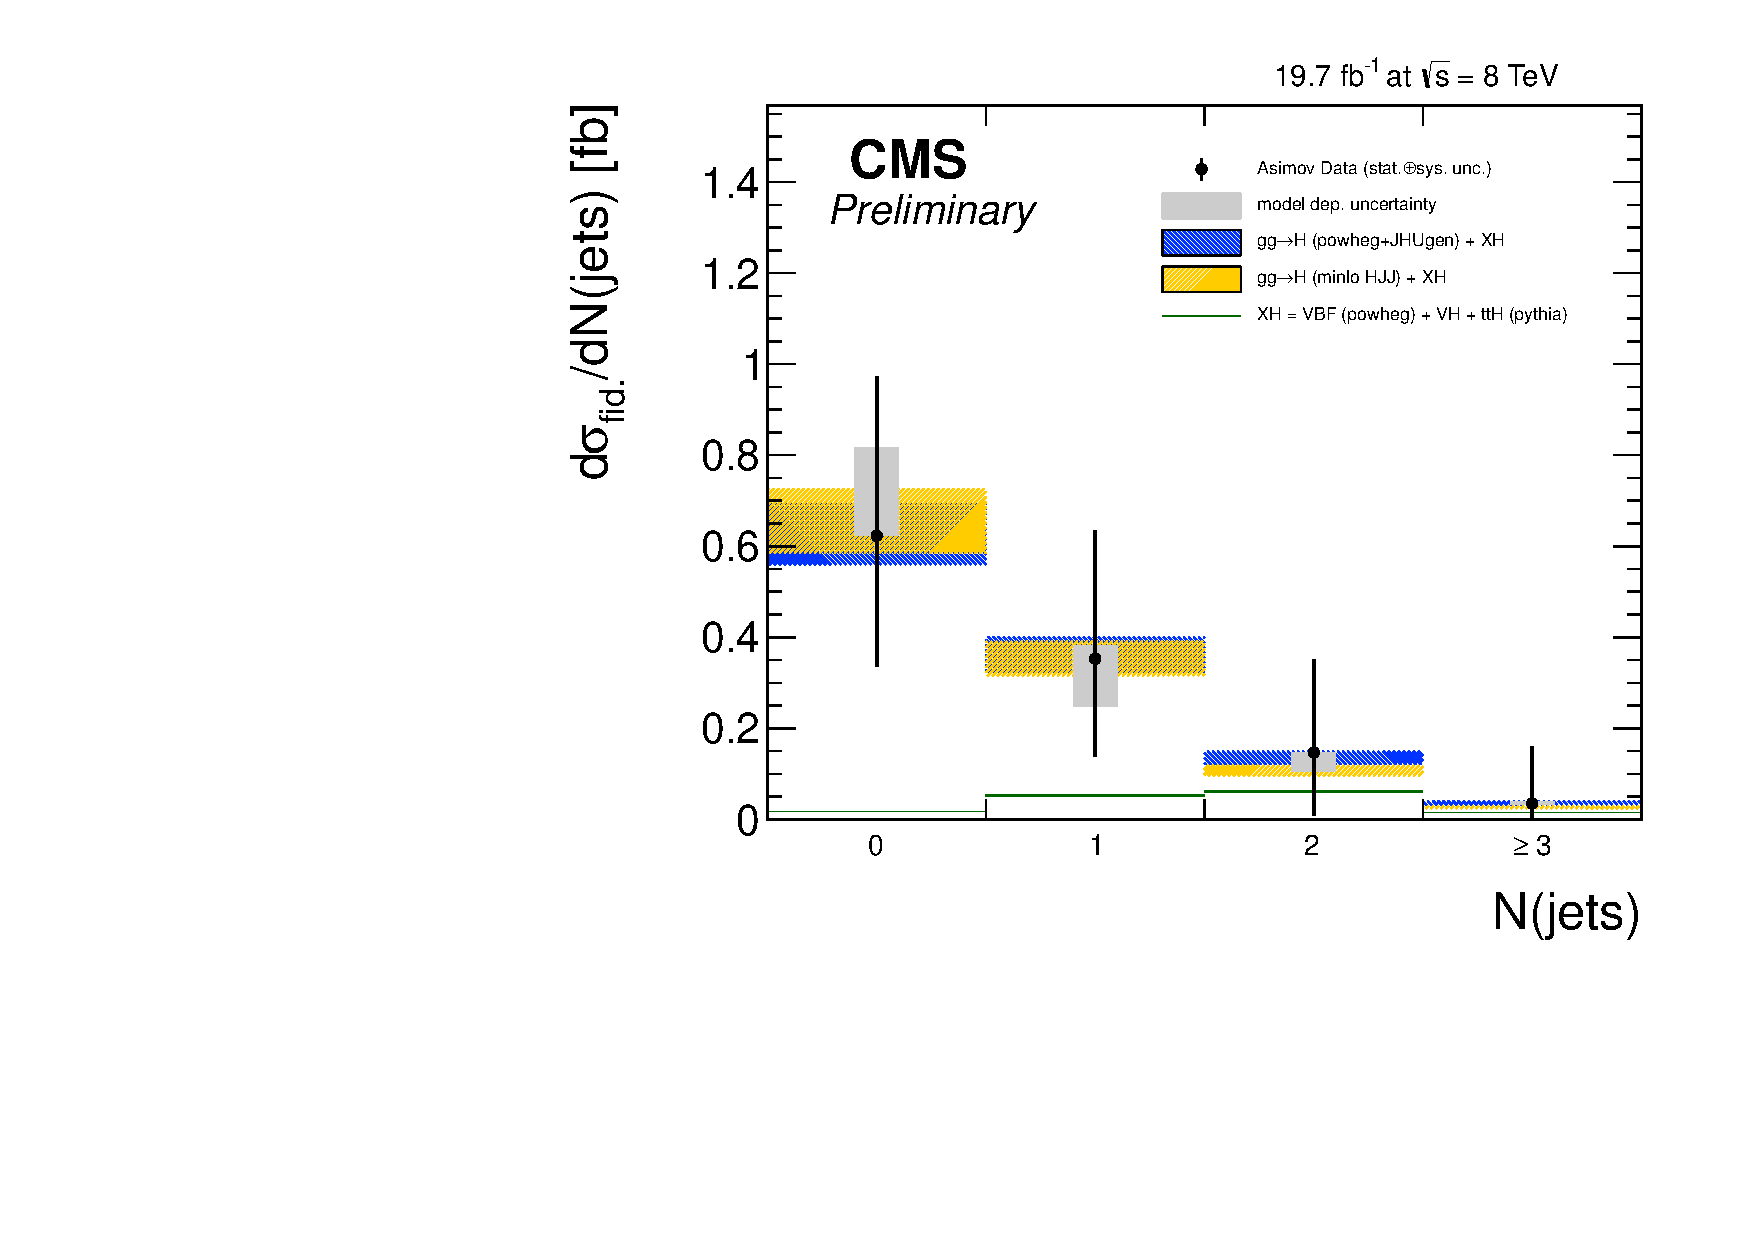
\includegraphics[width=0.48\textwidth,angle=0]{Plots/njets_reco_pt30_eta4p7_unfoldwith_ggH_powheg15_JHUgen_125_fixfrac.pdf}
      \label{fig:differential-results-fixfrac:d}
    }
    \caption{Results of the differential cross section measurement for different observables. The predictions from {\sc powheg+JHUgen} and {\sc minloHJJ} are shown in blue and yellow, respectively. The central value of the measurement is obtained using the efficiencies from the {\sc powheg+JHUgen} gg$\rightarrow$H model with m(H)= 125 $\GeV$, and the error bar represents the combined statistical and systematic uncertainty. The grey box represents the additional uncertainty incurred when using different models to unfold the observed data distribution back to particle level. The fraction of $4e,4\mu$ and $2e2\mu$ in each bin are fixed to their SM expectations.
    }
  \label{fig:differential-results-fixfrac}
 \end{center}
\end{figure}

